\let\negmedspace\undefined
\let\negthickspace\undefined
\documentclass[journal]{IEEEtran}
\usepackage[a5paper, margin=10mm, onecolumn]{geometry}
%\usepackage{lmodern} % Ensure lmodern is loaded for pdflatex
\usepackage{tfrupee} % Include tfrupee package

\setlength{\headheight}{1cm} % Set the height of the header box
\setlength{\headsep}{0mm}     % Set the distance between the header box and the top of the text

\usepackage{gvv-book}
\usepackage{gvv}
\usepackage{cite}
\usepackage{amsmath,amssymb,amsfonts,amsthm}
\usepackage{algorithmic}
\usepackage{graphicx}
\usepackage{textcomp}
\usepackage{xcolor}
\usepackage{txfonts}
\usepackage{listings}
\usepackage{enumitem}
\usepackage{mathtools}
\usepackage{gensymb}
\usepackage{comment}
\usepackage[breaklinks=true]{hyperref}
\usepackage{tkz-euclide} 
\usepackage{listings}
\def\inputGnumericTable{}                                 
\usepackage[latin1]{inputenc}                                
\usepackage{color}                                            
\usepackage{array}                                            
\usepackage{longtable}                                       
\usepackage{calc}                                             
\usepackage{multirow}                                         
\usepackage{hhline}                                           
\usepackage{ifthen}                                           
\usepackage{lscape}
\begin{document}

\bibliographystyle{IEEEtran}
\vspace{3cm}

\title{8.2.48}
\author{AI25BTECH11012 - GARIGE UNNATHI}
% \maketitle
% \newpage
% \bigskip
{\let\newpage\relax\maketitle}


\renewcommand{\thefigure}{\theenumi}
\renewcommand{\thetable}{\theenumi}
\setlength{\intextsep}{10pt} % Space between text and floats


\numberwithin{equation}{enumi}
\numberwithin{figure}{enumi}
\renewcommand{\thetable}{\theenumi}


\textbf{Question}:\\
Find the equation of the conic, that satisfies the given conditions. \\ 
focus (-1,-2) and directrix x - 2y + 3 = 0.
 
\textbf{Solution: }
Let :
\begin{align}
    \vec{F} = \myvec{-1\\-2}\\
    directrix \quad equation \quad is : \myvec{1\\-2}^{T}\vec{x} = -3
\end{align}
The equation of a conic with directrix $\vec{n}^{T}$$\vec{x}$ = c , eccentricity e and focus $\vec{F}$ is given by:
\begin{align}
    g(\vec{x}) = \vec{x}^{T}\vec{V}\vec{x} + 2\vec{u}^{T}\vec{x} + f  = 0
\end{align}

where :

\begin{align*}
\vec{V} = \lVert \vec{n} \rVert^{2}\vec{I} - e^{2}\vec{n}\vec{n}^{T} , \\
\vec{u} = ce^{2}\vec{n} - \lVert \vec{n} \rVert^{2}\vec{F} , \\
f = \lVert \vec{n} \rVert^{2}\lVert \vec{F} \rVert^{2} - c^{2}e^{2}
\end{align*}

From the question we can say that the conic is a parabola that is e = 1 ;\\
Calculating $\vec{V}$ ,$\vec{u}$ and f by using the above equations we get :
\begin{align}
   \vec{V} = \myvec{4 & 2\\2 & 1}\\
   \vec{u} = \myvec{2\\16}\\
   f = 16
\end{align}
Finding eigen values of $\vec{V}$ :
\begin{align}
    det\lvert \vec{V} - \lambda\vec{I} \rvert = 0\\
    \begin{vmatrix} 4 - \lambda & 2 \\ 2 & 1 - \lambda \end{vmatrix} = 0\\
    \lambda^2 - 5\lambda = 0\\
    \lambda = 5 \quad and \quad 0 
\end{align}
Eigen vectors $\vec{v}$ for any any square matrix $\vec{A}$ is defined as :
\begin{align}
    \vec{A}\vec{v} = \lambda\vec{v}\\
    (\vec{A} - \lambda)\vec{v} = 0 \\
    for \quad \lambda = 0 \quad v_1 = \myvec{1\\-2}\\
        for \quad \lambda = 5 \quad v_2 = \myvec{2\\1}
\end{align}

Substituting in the equation 0.3 we get the equation of the conic to be :
\begin{align}
  \vec{x}^{T}\myvec{4 & 2\\2 & 1}\vec{x} + 2\myvec{2 \\ 16}^{T}\vec{x} +16 =0
\end{align}





\begin{figure}[h!]
   \centering
   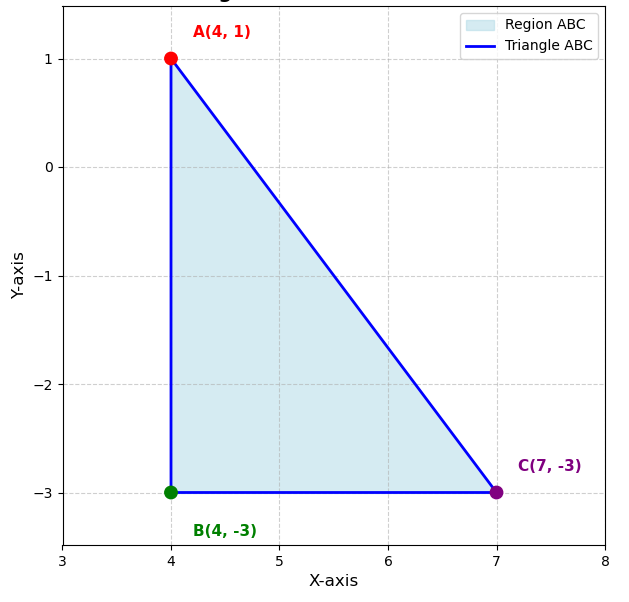
\includegraphics[width=0.7\linewidth]{/Users/unnathi/Documents/ee1030-2025/ai25btech11012/matgeo/8.2.48/figs/fig.png}
   \caption{}
   \label{stemplot}
\end{figure}





\end{document}
